%*************************************************************
% Author Name
%*************************************************************
%Chapter One
%*************************************************************
%*************************************************************
% Introduction
%*************************************************************
%*************************************************************
\chapter{Introduction}
\label{ch:intro}
%*************************************************************



%*************************************************************
\section{Sample Section}
\label{sec:ch1_section_one}
%*************************************************************
Add your text here. To make any citations, you need to import the bibtex of your reference to the 'Ref.bib' file. Then use the citekey \cite{nagothu2018microservice} to add your citations \cite{nagothu2021authenticating}.

You can refer to your figure usig \ref{fig:ch1_figure}. The the following commands to import the figures from 'figs' folder. Try to follow a naming convention for each figure based on their chapter appearance. If the figure is too big, then you can adjust its size by changing the 'width' parameter. 

\begin{figure}[t]
    \centering
        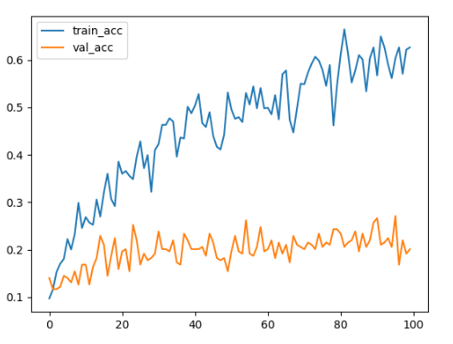
\includegraphics[width=0.98\textwidth]{figs/acc.png}
    \caption{A sample for figure.}
    \label{fig:ch1_figure}
    \vspace{-10pt}
\end{figure}


%*************************************************************
\section{Challenges and Motivation}
\label{sec:ch1_challenges}
%*************************************************************



%*************************************************************
\section{Major Contributions}
\label{sec:ch1_contributions}
%*************************************************************
 A summary of the contributions made in this dissertation is as follows,

\begin{itemize}
    \item A comprehensive study of existing techniques
    \item Item 2
    \item Item 3
    
\end{itemize}

%*************************************************************
% End of Introduction
%*************************************************************
%*************************************************************
